\section{格林公式}
\subsection{格林公式}
在一元函数积分学中,牛顿--莱布尼茨公式\[
\int_a^b f(x) \dd{x} = F(b) - F(a)
\]表示:\(f(x)\)在区间\([a,b]\)上的积分可以通过它的原函数\(F(x)\)在这个区间端点上的值来表达.

下面要介绍的格林公式告诉我们,在平面闭区域\(D\)上的二重积分可以通过沿闭区域\(D\)的边界曲线\(L\)上的曲线积分来表达.

\begin{definition}\label{definition:线积分与面积分.平面闭区域的边界曲线的取向}
对于平面区域\(D\)的边界曲线\(C = \partial D\),我们规定\(C\)的方向如下:

设坐标平面的\(x\)轴、\(y\)轴对应的基向量分别为\(\mat{e}_x\)和\(\mat{e}_y\),令\(\mat{e}_z = \mat{e}_x \times \mat{e}_y\).任取点\(P \in C\),则可得与曲线切于点\(P\)的直线\(L\).

在点\(P\)取一个半径\(r\)足够小的去心邻域,使得其与区域\(D\)的内部的交集\(I(D) \cap \mathring{U}(P,r)\)是单连通区域,再从中任取一点\(Q\),即\[
Q \in I(D) \cap \mathring{U}(P,r).
\]

任意取一个与直线\(L\)平行的单位向量\(\mat{e}_L\).令\(\Phi = (\mat{e}_z \times \mat{e}_L) \cdot \vec{PQ}\).
如果\[
\Phi < 0,
\]则称单位向量\(\mat{e}_L\)的方向为曲线\(C\)在点\(P\)处的正方向;反之,如果\[
\Phi > 0,
\]则称单位向量\(\mat{e}_L\)的方向为曲线\(C\)在点\(P\)处的负方向.
\end{definition}
如\cref{figure:线积分与面积分.平面区域的边界曲线与其取向},平面区域\(D\)的边界是曲线\(L\)和曲线\(l\)的并集\(L+l\).曲线\(L\)的正向是它的逆时针方向(记作\(L^+\)),其负向是它的顺时针方向(记作\(L^-\));曲线\(l\)的正向是它的顺时针方向(记作\(l^+\)),其负向是它的逆时针方向(记作\(l^-\));总的来说,平面区域\(D\)的正向边界曲线就是\((L^+ + l^+)\).

\begin{figure}[ht]
\centering
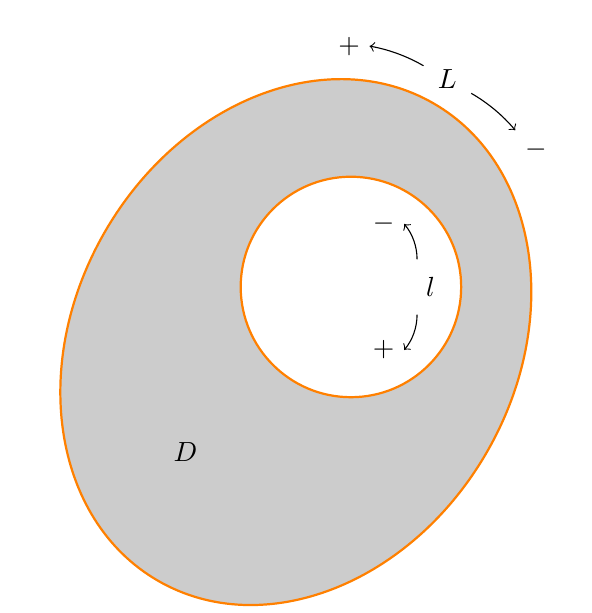
\begin{tikzpicture}[scale=.7]
	\draw[orange,fill=gray!40,rotate=60,thick] (0,0)ellipse[x radius=5,y radius=4];
	\draw[orange,fill=white,thick] (1,1)ellipse[x radius=2,y radius=2];
	\draw (-2,-2)node{\(D\)};
	\begin{scope}[rotate=60]
		\coordinate (P1) at (5.5,0);
		\draw (P1)node{\(L\)};
		\draw[->] (P1)+(0,.5) arc[start angle=0,end angle=20,radius=3]node[left]{\(+\)};
		\draw[->] (P1)+(0,-.5) arc[start angle=0,end angle=-20,radius=3]node[below right]{\(-\)};
	\end{scope}
	\begin{scope}
		\coordinate (P2) at (2.7,1);
		\draw (P2)node[left]{\(l\)};
		\draw[->] (P2)+(-.5,.5) arc[start angle=0,end angle=40,radius=1]node[left]{\(-\)};
		\draw[->] (P2)+(-.5,-.5) arc[start angle=0,end angle=-40,radius=1]node[left]{\(+\)};
	\end{scope}
\end{tikzpicture}
\caption{平面区域的边界曲线与其取向}
\label{figure:线积分与面积分.平面区域的边界曲线与其取向}
\end{figure}

\begin{theorem}[格林公式]
设闭区域\(D\)由分段光滑的曲线\(L\)围成,函数\(P(x,y)\)和\(Q(x,y)\)在\(D\)上具有一阶连续偏导数,则有
\begin{equation}\label{equation:线积分与面积分.格林公式}
\iint_D \left( \pdv{Q}{x} - \pdv{P}{y} \right) \dd{x}\dd{y}
= \oint_L P\dd{x} + Q\dd{y},
\end{equation}其中\(L\)是\(D\)的取正向的边界曲线.
\end{theorem}
\cref{equation:线积分与面积分.格林公式}叫做\DefineConcept{格林公式}.

下面说明格林公式的一个简单应用.
在格林公式中,令\(P=-y\)、\(Q=x\),可得\[
2 \iint_D \dd{x}\dd{y}
=\oint_L x\dd{y}-y\dd{x}.
\]上式左端是闭区域\(D\)的面积\(A\)的两倍,因此有
\begin{equation}\label{equation:线积分与面积分.利用格林公式计算闭区域的面积}
A = \frac{1}{2} \oint_L x\dd{y}-y\dd{x}.
\end{equation}
\begin{example}
求椭圆\(x = a \cos\theta, y = b \sin\theta\)所围成图形的面积\(A\).
\begin{solution}
根据\cref{equation:线积分与面积分.利用格林公式计算闭区域的面积} 有\begin{align*}
A &= \frac{1}{2} \oint_L x\dd{y}-y\dd{x} \\
&= \frac{1}{2} \int_0^{2\pi} \left[ a \cos\theta \cdot b \cos\theta \dd{\theta}
	- b \sin\theta \cdot (-a \sin\theta) \dd{\theta} \right] \\
&= \frac{1}{2} ab \int_0^{2\pi} \dd{\theta}
= \pi ab.
\end{align*}
\end{solution}
\end{example}

\begin{example}
计算\(\oint_L \frac{x\dd{y}-y\dd{x}}{x^2+y^2}\),其中\(L\)是一条不经过原点的分段光滑的若尔当闭曲线,\(L\)的方向为逆时针方向.
\begin{solution}
记\(P = -\frac{y}{x^2+y^2}, Q = \frac{x}{x^2+y^2}\).
当\(x^2+y^2\neq0\)时,有\[
\pdv{Q}{x} = \frac{y^2-x^2}{(x^2+y^2)^2} = \pdv{P}{y}.
\]记\(L\)所围成的闭区域为\(D\).

当\(\opair{0,0} \notin D\)时,由\cref{equation:线积分与面积分.格林公式} 有\[
\oint_L \frac{x\dd{y}-y\dd{x}}{x^2+y^2} = \iint_D 0 \dd{x}\dd{y} = 0;
\]

当\(\opair{0,0} \in D\)时,取\(r>0\)使得\(\Set{ \opair{x,y} \given x^2+y^2 \leq r^2 } \subseteq D\).作圆\(l: x^2+y^2=r^2\),记\(L\)和\(l\)所围成的闭区域为\(D_1\).
对复连通区域\(D_1\)应用格林公式,得\[
\oint_L \frac{x\dd{y}-y\dd{x}}{x^2+y^2} - \oint_l \frac{x\dd{y}-y\dd{x}}{x^2+y^2}
= \iint_{D_1} 0 \dd{x}\dd{y} = 0,
\]其中\(l\)的方向取逆时针方向.
于是\[
\oint_L \frac{x\dd{y}-y\dd{x}}{x^2+y^2}
= \oint_l \frac{x\dd{y}-y\dd{x}}{x^2+y^2}
= \int_0^{2\pi} \frac{r^2 \cos^2\theta + r^2 \sin^2\theta}{r^2} \dd{\theta}
= 2\pi.
\]
\end{solution}
\end{example}

\begin{example}[二维格林第一公式、二维格林第二公式]
设\(u(x,y)\)、\(v(x,y)\)在闭区域\(D\)上都具有二阶连续偏导数,分段光滑的曲线\(L\)为\(D\)的正向边界曲线.证明:\begin{gather}
\iint_D v \laplacian{u} \dd{x}\dd{y} = - \iint_D (\grad u \cdot \grad v) \dd{x}\dd{y} + \oint_L v \pdv{u}{\mat{n}} \dd{s};
\label{equation:线积分与面积分.二维格林第一公式} \\
\iint_D (u \laplacian v - v \laplacian u) \dd{x}\dd{y} = \oint_L \left( u \pdv{v}{\mat{n}} - v \pdv{u}{\mat{n}} \right) \dd{s},
\label{equation:线积分与面积分.二维格林第二公式}
\end{gather}其中\(\pdv{u}{\mat{n}}\)、\(\pdv{v}{\mat{n}}\)分别是\(u\)、\(v\)沿\(L\)的外法线向量\(\mat{n}\)的方向导数,二维拉普拉斯算子\(\laplacian = \pdv[2]{x} + \pdv[2]{y}\).
\begin{proof}
因为方向导数\[
\pdv{u}{\mat{n}}
= \pdv{u}{x} \cos\alpha
+ \pdv{u}{y} \cos\beta,
\qquad
\pdv{v}{\mat{n}}
= \pdv{v}{x} \cos\alpha
+ \pdv{v}{y} \cos\beta,
\]其中\(\cos\alpha\)、\(\cos\beta\)是\(L\)在点\(\opair{x,y}\)处的外法线向量的方向余弦,那么\(L\)在该点处的正向单位切向量为\(\mat{\tau} = \opair{-\cos\beta,\cos\alpha}\),于是利用格林公式可得\begin{align*}
\oint_L v \pdv{u}{\mat{n}} \dd{s}
&= \oint_L v \left(
\pdv{u}{x} \cos\alpha
+ \pdv{u}{y} \cos\beta
\right) \dd{s} \\
&= \oint_L \left( - v \pdv{u}{y} \right) \dd{x} + \left( v \pdv{u}{x} \right) \dd{y} \\
&= \iint_D \left[ \pdv{x} \left( v \pdv{u}{x} \right) - \pdv{y} \left( - v \pdv{u}{y} \right) \right] \dd{x}\dd{y} \\
&= \iint_D \left( \pdv{v}{x} \pdv{u}{x} + v \pdv[2]{u}{x} + \pdv{v}{y} \pdv{u}{y} + v \pdv[2]{u}{y} \right) \dd{x}\dd{y} \\
&= \iint_D (\grad u \cdot \grad v) \dd{x}\dd{y} + \iint_D v \laplacian{u} \dd{x}\dd{y},
\end{align*}移项可得\cref{equation:线积分与面积分.二维格林第一公式}.而\cref{equation:线积分与面积分.二维格林第二公式} 可由\cref{equation:线积分与面积分.二维格林第一公式} 推得,故略去.
\end{proof}
\end{example}

\begin{example}
设函数\(f(x,y)\)在区域\(D=\Set{\opair{x,y} \given x^2+y^2\leq1}\)上具有二阶连续偏导数,且\(\pdv[2]{f}{x}+\pdv[2]{f}{y}=e^{-(x^2+y^2)}\),求二重积分\(I=\iint_D\left(x\pdv{f}{x}+y\pdv{f}{y}\right)\dd{x}\dd{y}\).
\begin{solution}
考虑区域\(D\)的形状,将积分\(I\)化为在极坐标系下的积分,令\(x=\rho\cos\theta, y=\rho\sin\theta\):\begin{align*}
I &= \int_0^1 \rho\dd{\rho} \int_0^{2\pi} \left(\rho\cos\theta\pdv{f}{x}+\rho\sin\theta\pdv{f}{y}\right) \dd{\theta} \\
&= \int_0^1 \rho\dd{\rho} \int_0^{2\pi} \left[\pdv{f}{x}\dd(\rho\sin\theta)-\pdv{f}{y}\dd(\rho\cos\theta)\right].
\end{align*}
考虑到\(\dd{x}=\dd(\rho\cos\theta), \dd{y}=\dd(\rho\sin\theta)\),所以\[
I = \int_0^1 \rho\dd{\rho} \oint_{L_{\rho}: x^2+y^2=\rho^2} \pdv{f}{x}\dd{y}-\pdv{f}{y}\dd{x}.
\]应用\hyperref[equation:线积分与面积分.格林公式]{格林公式},则有\begin{align*}
\oint_{L_{\rho}: x^2+y^2=\rho^2} \pdv{f}{x}\dd{y}-\pdv{f}{y}\dd{x}
&= \iint_{D_{\rho}: x^2+y^2\leq\rho^2} \left(\pdv[2]{f}{x}+\pdv[2]{f}{y}\right) \dd{\sigma} \\
&= \iint_{D_{\rho}: x^2+y^2\leq\rho^2} e^{-(x^2+y^2)} \dd{\sigma} \\
&= \int_0^{2\pi} \dd{\theta} \int_0^{\rho} e^{-\rho^2} \rho\dd{\rho} \\
&= \pi \left(1-e^{-\rho^2}\right).
\end{align*}
那么\[
I = \int_0^1 \pi \left(1-e^{-\rho^2}\right) \rho\dd{\rho}
=  \frac{\pi}{2e}.
\]
\end{solution}
\end{example}

\subsection{平面上曲线积分与路径无关的条件}
在物理上(特别是力学中)要研究所谓“势场”,就是要研究场力所作的功与路径无关的情形.
在什么条件下场力所作的功与路径无关?
这个问题在数学上就是要研究曲线积分与路径无关的条件.
为了研究这个问题,先要明确什么叫做“曲线积分\(\int_L P\dd{x}+Q\dd{y}\)与路径无关”.
\begin{definition}
设\(G\)是一个区域,\(P(x,y)\)以及\(Q(x,y)\)在区域\(G\)内具有一阶连续偏导数.
如果对于\(G\)内任意指定的两个点\(A\)、\(B\)
以及\(G\)内从点\(A\)到点\(B\)的任意两条曲线\(L_1\)、\(L_2\),
等式\[
\int_{L_1}{P\dd{x}+Q\dd{y}}
=\int_{L_2}{P\dd{x}+Q\dd{y}}
\]恒成立,
就说“曲线积分\(\int_L P\dd{x}+Q\dd{y}\)在\(G\)内与路径无关”,
否则便说“曲线积分\(\int_L P\dd{x}+Q\dd{y}\)在\(G\)内与路径相关”.
\end{definition}
“曲线积分\(\int_L P\dd{x}+Q\dd{y}\)在\(G\)内与路径无关”相当于“沿\(G\)内任意闭曲线\(C\)的曲线积分\(\oint_C P\dd{x}+Q\dd{y}\)等于零”.

\begin{theorem}\label{theorem:线积分与面积分.平面上曲线积分与路径无关的充要条件}
设区域\(G\)是一个单连通域,函数\(P(x,y)\)、\(Q(x,y)\)在\(G\)内具有一阶连续偏导数,那么曲线积分\(\int_L P\dd{x}+Q\dd{y}\)在\(G\)内与路径无关(或沿\(G\)内任意闭曲线的曲线积分为零)的充要条件是:\[
\pdv{P}{y}=\pdv{Q}{x}
\]在\(G\)内恒成立.
\end{theorem}
如果\cref{theorem:线积分与面积分.平面上曲线积分与路径无关的充要条件} 所要求的两个条件“区域\(G\)是单连通区域,且函数\(P(x,y)\)和\(Q(x,y)\)在\(G\)内具有一阶连续偏导数”不能同时满足,那么定理的结论不能保证成立.
例如当区域\(G\)中出现破坏函数\(P\)、\(Q\)及\(\pdv{Q}{x}\)、\(\pdv{P}{y}\)连续性条件的\DefineConcept{奇点}时,定理的结论就不能保证成立.

\subsection{二元函数的全微分求积}
\begin{theorem}\label{theorem:线积分与面积分.二元函数的全微分的存在条件}
设区域\(G\)是一个单连通区域.
函数\(P(x,y)\)、\(Q(x,y)\)在\(G\)内具有一阶连续偏导数.
则\(P(x,y)\dd{x}+Q(x,y)\dd{y}\)在\(G\)内为某一函数\(u(x,y)\)的全微分的充要条件是\[
\pdv{P}{y}=\pdv{Q}{x}
\]在\(G\)内恒成立.
\end{theorem}

根据\cref{theorem:线积分与面积分.平面上曲线积分与路径无关的充要条件} 和\cref{theorem:线积分与面积分.二元函数的全微分的存在条件},立即可得如下推论.
\begin{corollary}
设区域\(G\)是一个单连通区域.
函数\(P(x,y)\)、\(Q(x,y)\)在\(G\)内具有一阶连续偏导数.
则曲线积分\(\int_L{P\dd{x}+Q\dd{y}}\)在\(G\)内与路径无关的充要条件是:
在\(G\)内存在函数\(u(x,y)\),使\(\dd{u}=P\dd{x}+Q\dd{y}\).
\end{corollary}

\subsection{曲线积分的基本定理}
\begin{definition}
若曲线积分\(\int_L \mat{F}\cdot\dd{\mat{r}}\)在区域\(G\)内与积分路径无关,则称向量场\(\mat{F}\)为\DefineConcept{保守场}.
\end{definition}

下面的定理给出了平面曲线积分与路径无关的另一种形式的条件,并为计算保守场中的曲线积分提供了一种简便的方法.
\begin{theorem}[曲线积分的基本定理]\label{theorem:线积分与面积分.曲线积分的基本定理}
设\(\mat{F}(x,y)=P(x,y)\mat{i}+Q(x,y)\mat{j}\)是平面区域\(G\)内的一个向量场,
\(P(x,y)\)、\(Q(x,y)\)都在\(G\)内连续,且存在一个数量函数\(f(x,y)\),
使得\(\mat{F}=\grad{f}\),
则曲线积分\(\int_L{\mat{F}\cdot\dd{\mat{r}}}\)在\(G\)内与路径无关,且
\begin{equation}\label{equation:线积分与面积分.曲线积分的基本公式}
\int_L \mat{F} \cdot \dd{\mat{r}}
= f(B)-f(A),
\end{equation}
其中\(L\)是位于\(G\)内起点为\(A\)、终点为\(B\)的任一分段光滑曲线.
\end{theorem}
\cref{theorem:线积分与面积分.曲线积分的基本定理} 表明,对于势场\(\mat{F}\),曲线积分\(\int_L \mat{F}\cdot\dd{\mat{r}}\)的值仅依赖于它的势函数\(f\)在路径\(L\)的两端点的值,而不依赖于两点间的路径,即积分\(\int_L \mat{F}\cdot\dd{\mat{r}}\)在\(G\)内与路径无关.
也就是说:势场是保守场.

\cref{equation:线积分与面积分.曲线积分的基本公式}
是与微积分基本公式\[
\int_a^b f(x) \dd{x}
= F(b) - F(a)
\](其中\(F'(x) = f(x)\))完全类似的向量微积分的相应公式,
称为\DefineConcept{曲线积分的基本公式}.
